\documentclass{beamer}
\input{../utils/preamble}
\createdgmtitle{6}
%--------------------------------------------------------------------------------
\begin{document}
%--------------------------------------------------------------------------------
\begin{frame}[noframenumbering,plain]
	\titlepage
	\resetonslide
\end{frame}
%=======

\begin{frame}{Recap of Previous Lecture}
	\begin{block}{Likelihood-Free Learning}
		\begin{itemize}
			\item Likelihood isn't a perfect metric for generative models.
			\item Likelihood may be intractable.
		\end{itemize}
	\end{block}
	Imagine we have two sets of samples:
	\begin{itemize}
		\item $\{\bx_i\}_{i=1}^{n_1} \sim \pd(\bx)$ -- real samples;
		\item $\{\bx_i\}_{i=1}^{n_2} \sim \pt(\bx)$ -- generated (fake) samples.
	\end{itemize}
	\[
		p(y = 1 | \bx) = P(\bx \sim \pd(\bx)); \quad p(y = 0 | \bx) = P(\bx \sim \pt(\bx))
	\]
	\vspace{-0.5cm}
	\begin{block}{Assumption}
		The generative distribution $\pt(\bx)$ matches the true distribution $\pd(\bx)$ if we can't distinguish between them using a discriminative model $p(y|\bx)$.
	\end{block}
	\begin{itemize}
		\item \textbf{Generator:} a generative model $\bx = \bG(\bz)$ that produces more realistic samples.
		\item \textbf{Discriminator:} a classifier $D(\bx) \in [0, 1]$ distinguishing real from generated samples.
	\end{itemize}
\end{frame}
%=======
\begin{frame}{Recap of Previous Lecture}
	\myfootnotewithlink{https://arxiv.org/abs/1406.2661}{Goodfellow I. J. et al. Generative Adversarial Networks, 2014}
	\begin{block}{GAN Optimality Theorem}
		The minimax game
		\[
		\min_{G} \max_D \Bigl[ \underbrace{\bbE_{\pd(\bx)} \log D(\bx) + \bbE_{p(\bz)} \log (1 - D(\bG(\bz)))}_{V(G, D)} \Bigr]
		\]
		has a global optimum at $\pd(\bx) = \pt(\bx)$, and then $D^*(\bx) = 0.5$.
	\end{block}
	\vspace{-0.3cm}
	\[
		\min_{G} V(G, D^*) = \min_{G} \left[ 2 \JSD(\pi \| p) - \log 4 \right] = -\log 4, \quad \pd(\bx) = \pt(\bx).
	\]
	If the generator can be \textbf{any} function and the discriminator is \textbf{optimal} at each step, then the generator is \textbf{guaranteed to converge} to the data distribution.  
\end{frame}
%=======
\begin{frame}{Recap of Previous Lecture}
	\myfootnotewithlink{https://arxiv.org/abs/1406.2661}{Goodfellow I. J. et al. Generative Adversarial Networks, 2014}
	\begin{itemize}
		\item The generator is updated in the parameter space; the discriminator isn't optimal at every iteration.
		\item Both generator and discriminator loss typically oscillate during GAN training.
	\end{itemize}
	\begin{block}{Objective}
		\vspace{-0.5cm}
		\[
		\min_{\btheta} \max_{\bphi} \left[ \bbE_{\pd(\bx)} \log D_{\bphi}(\bx) + \bbE_{p(\bz)} \log (1 - D_{\bphi}(\bG_{\btheta}(\bz))) \right]
		\]
		\vspace{-0.5cm}
	\end{block}
	\begin{figure}
		\centering
		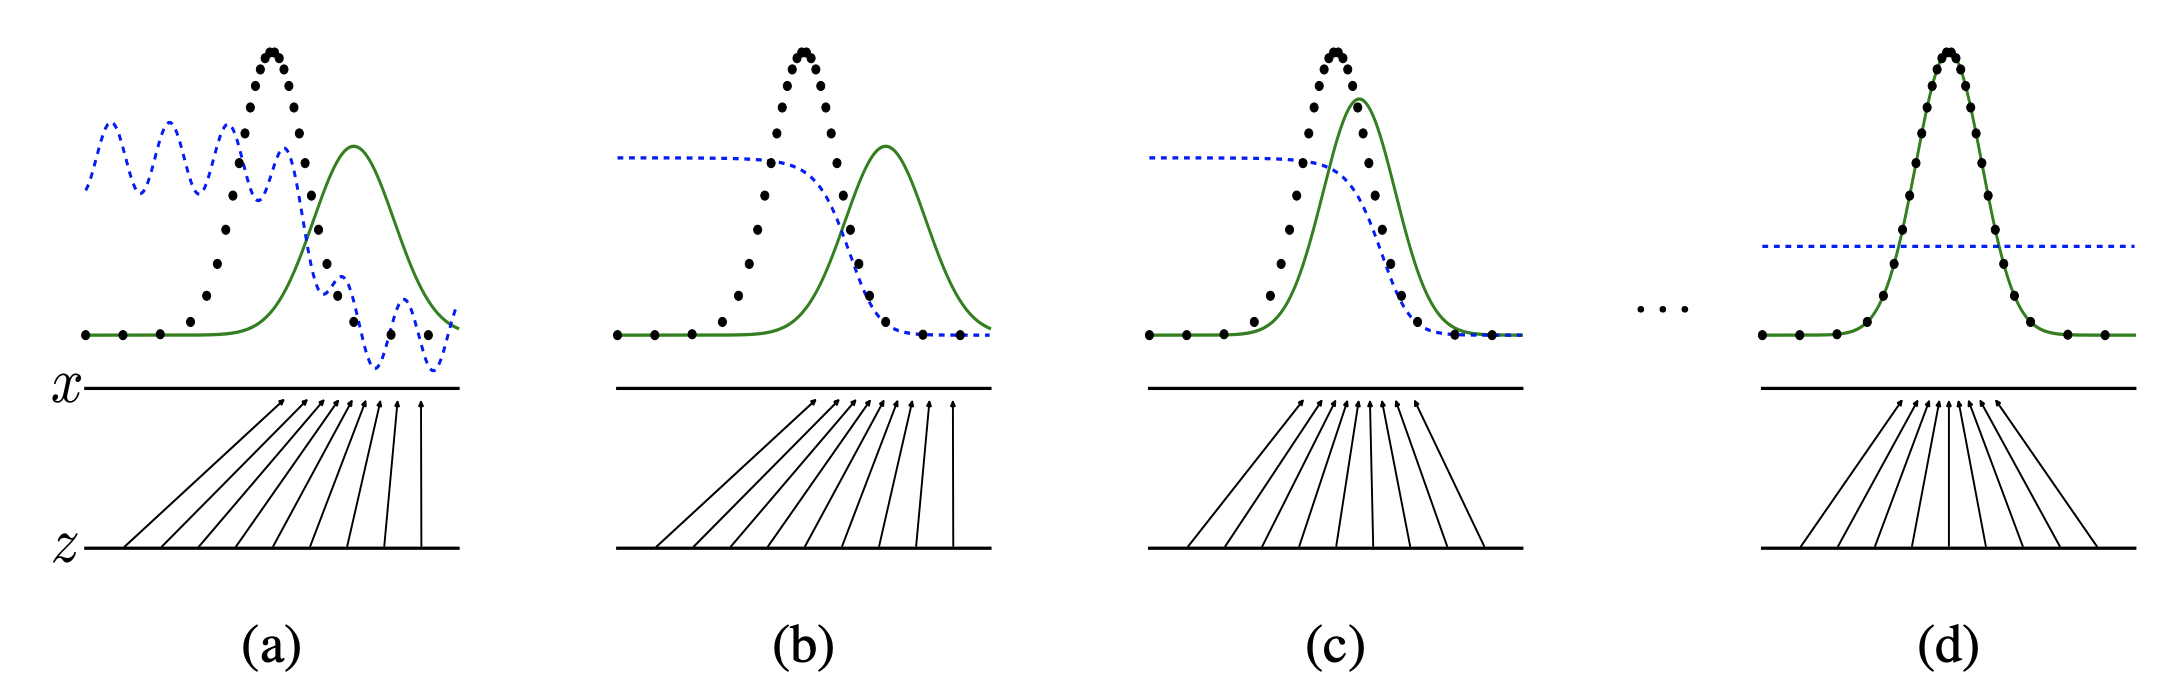
\includegraphics[width=1.0\linewidth]{figs/gan_1}
	\end{figure}
\end{frame}
%=======
\begin{frame}{Recap of Previous Lecture}
	\myfootnote{\href{https://arxiv.org/abs/1406.2661}{Goodfellow I. J. et al. Generative Adversarial Networks, 2014} \\
		\href{https://arxiv.org/abs/1701.04862}{Arjovsky M., Bottou L. Towards Principled Methods for Training Generative Adversarial Networks, 2017}}
	\begin{block}{Main Issues With Standard GANs}
		\begin{itemize}
			\item Vanishing gradients (solution: non-saturating GAN).
			\item Mode collapse (arises from Jensen-Shannon divergence).
		\end{itemize}
	\end{block}
	\begin{block}{Standard GAN}
		\vspace{-0.2cm}
		\[
		\min_{\btheta} \max_{\bphi} \left[ \bbE_{\pd(\bx)} \log D_{\bphi}(\bx) + \bbE_{p(\bz)} \log (1 - D_{\bphi}(\bG_{\btheta}(\bz))) \right]
		\]
		\vspace{-0.4cm}
	\end{block}
	\vspace{-0.1cm}
	\begin{block}{Informal Theoretical Results}
		Both the data distribution $\pd(\bx)$ and the generative distribution $\pt(\bx)$ are low-dimensional with disjoint supports. In such cases,
		\[
			\KL(\pd \| \pt) = \KL(\pt \| \pd) = \infty, \quad \JSD(\pd \| \pt) = \log 2.
		\]
	\end{block}
\end{frame}
%=======
\begin{frame}{Recap of Previous Lecture}
	\myfootnotewithlink{https://udlbook.github.io/udlbook/}{Simon J.D. Prince. Understanding Deep Learning, 2023}
	\begin{figure}
		\centering
		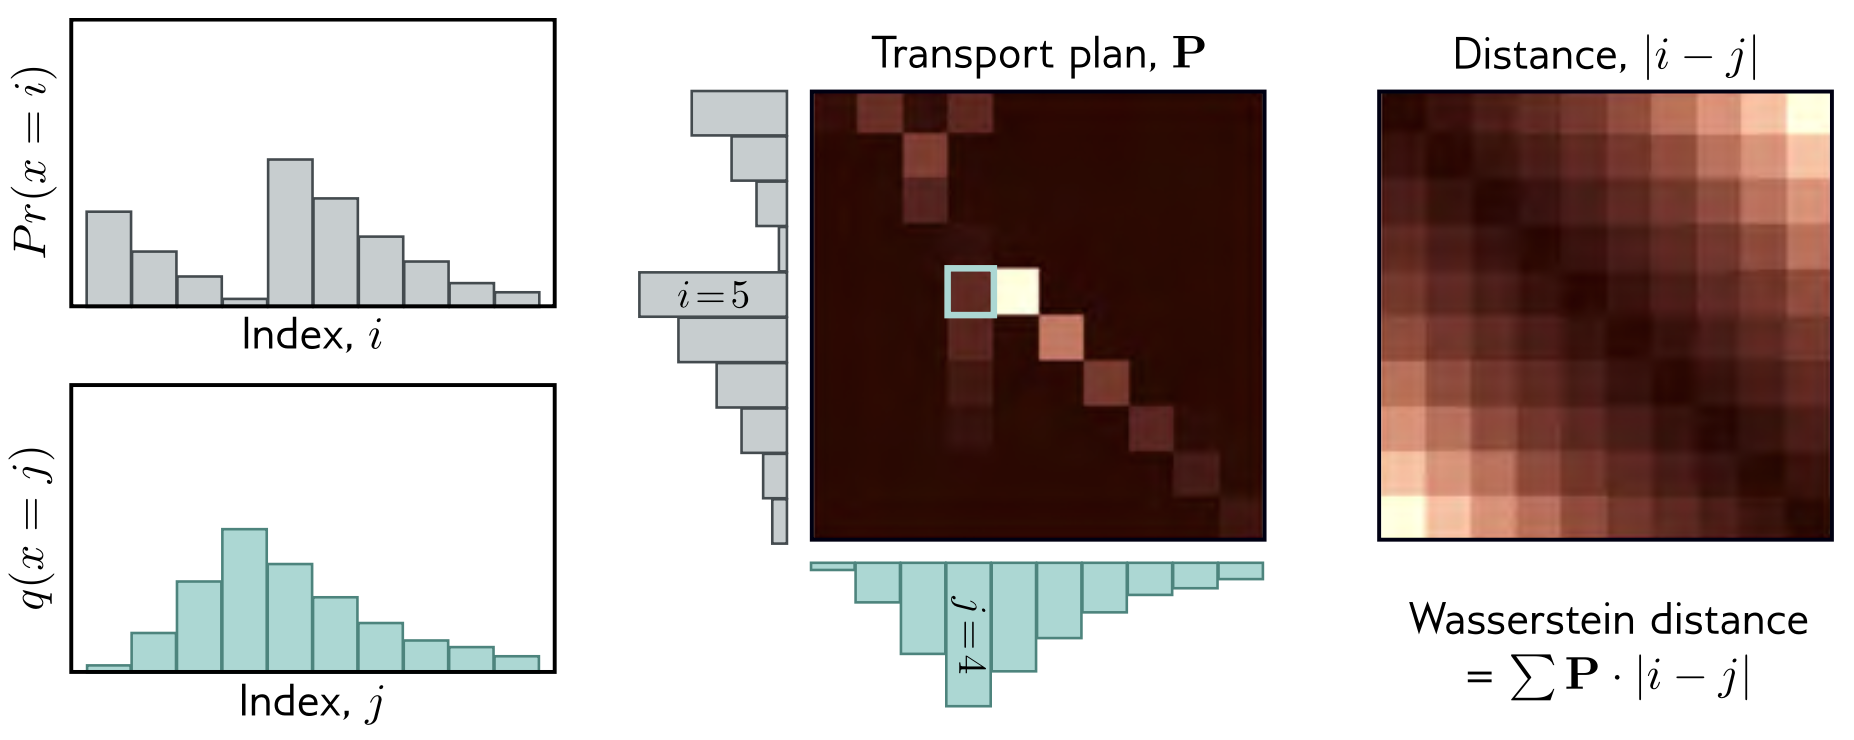
\includegraphics[width=0.8\linewidth]{figs/discrete_wasserstein}
	\end{figure}
	\vspace{-0.3cm}
	\begin{block}{Wasserstein Distance}
		\vspace{-0.7cm}
		{\small
		\[
		W(\pi \| p) = \inf_{\gamma \in \Gamma(\pi, p)} \bbE_{(\bx_1, \bx_2) \sim \gamma} \| \bx_1 - \bx_2 \| =  \inf_{\gamma \in \Gamma(\pi, p)} \int \| \bx_1 - \bx_2 \| \gamma (\bx_1, \bx_2) d \bx_1 d \bx_2
		\]
		}
		\vspace{-0.5cm}
		\begin{itemize}
			\item $\gamma(\bx_1, \bx_2)$ -- transportation plan (amount of "dirt" to transport from $\bx_1$ to $\bx_2$).
			\item $\Gamma(\pi, p)$ -- set of all joint distributions $\gamma (\bx_1, \bx_2)$ with marginals $\pi$ and $p$ ($\int \gamma(\bx_1, \bx_2) d \bx_1 = p(\bx_2)$, $\int \gamma(\bx_1, \bx_2) d \bx_2 = \pi(\bx_1)$).
			\item $\gamma(\bx_1, \bx_2)$ -- the amount; $\|\bx_1 - \bx_2 \|$ -- the distance.
		\end{itemize}
	\end{block}
\end{frame}
%=======
\begin{frame}{Recap of Previous Lecture}
	\myfootnotewithlink{https://arxiv.org/abs/1701.07875}{Arjovsky M., Chintala S., Bottou L. Wasserstein GAN, 2017}
	\begin{block}{Theorem (Kantorovich-Rubinstein Duality)}
		\vspace{-0.2cm}
		\[
		W(\pd \| \pt) = \frac{1}{K} \max_{\| f \|_L \leq K} \left[ \bbE_{\pd(\bx)} f(\bx)  - \bbE_{\pt(\bx)} f(\bx)\right],
		\]
		where $\| f \|_L \leq K$ denotes $K$-Lipschitz continuous functions.
	\end{block}
	\begin{block}{WGAN Objective}
		\vspace{-0.5cm}
		\[
		\min_{\btheta} {\color{violet}W(\pd \| \pt)} = \min_{\btheta} {\color{violet}\max_{\bphi \in \boldsymbol{\Phi}} \left[ \bbE_{\pd(\bx)} f_{\bphi}(\bx)  - \bbE_{p(\bz)} f_{\bphi}(\bG_{\btheta}(\bz))\right]}.
		\]
		\vspace{-0.5cm}
	\end{block}
	\begin{itemize}
		\item The function $f$ in WGAN is called the \textit{critic}.
		\item If parameters $\bphi$ lie in a compact set $\boldsymbol{\Phi} \in [-c, c]^d$, then $f(\bx, \bphi)$ is $K$-Lipschitz continuous. 
	\end{itemize}
	\begin{multline*}
		K \cdot W(\pd \| \pt) = \max_{\| f \|_L \leq K} \left[ \bbE_{\pd(\bx)} f(\bx) - \bbE_{\pt(\bx)} f(\bx)\right] \geq 
		\\ \geq \max_{\bphi \in \boldsymbol{\Phi}} \left[ \bbE_{\pd(\bx)} f_{\bphi}(\bx)  - \bbE_{\pt(\bx)} f_{\bphi}(\bx)\right]
	\end{multline*}
\end{frame}
%=======
\begin{frame}{Outline}
	\tableofcontents
\end{frame}
%=======
\section{Evaluation of Likelihood-Free Models}
%=======
\begin{frame}{Evaluation of Likelihood-Free Models}
\myfootnotewithlink{https://deepgenerativemodels.github.io}{image credit: https://deepgenerativemodels.github.io}
	\begin{block}{Likelihood-Based Models}
		\begin{itemize}
			\item \textbf{Train:} fit the model.
			\item \textbf{Validation:} tune hyperparameters.
			\item \textbf{Test:} assess generalization by reporting likelihood.
		\end{itemize}
	\end{block}
	\eqpause
	Not all models have tractable likelihoods \\ (VAE: compare ELBO values; GAN: \textbf{???}).
	\eqpause
	\begin{block}{Desirable Properties for Samples}
		\begin{itemize}
			\item Sharpness
			\begin{figure}
				\centering
				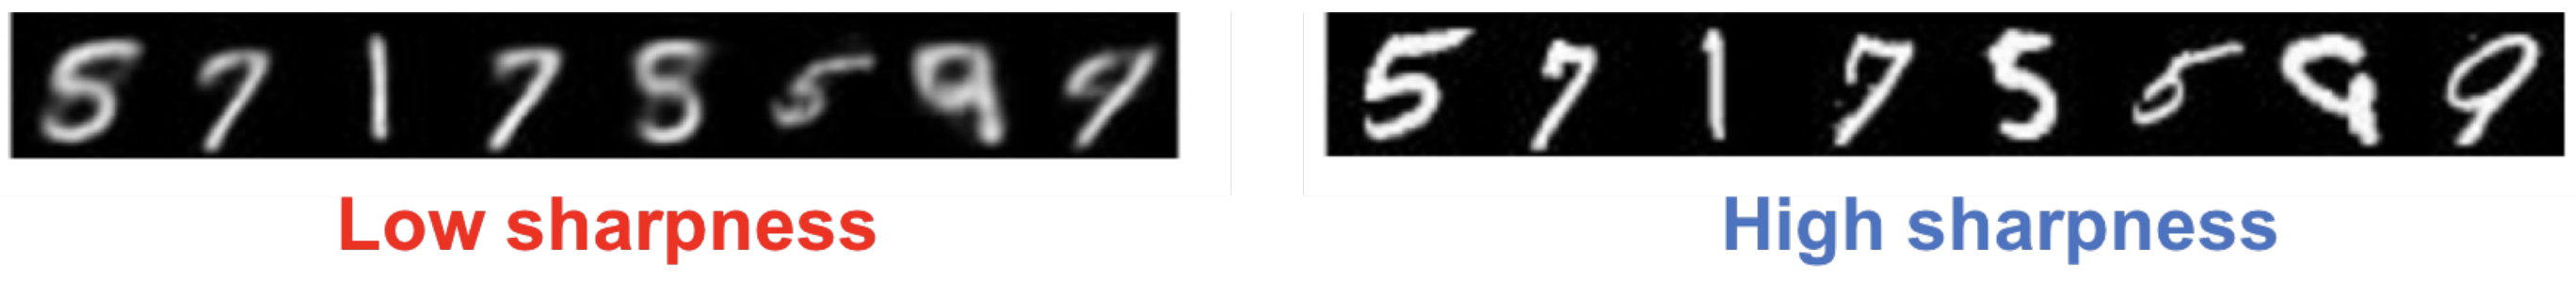
\includegraphics[width=0.9\linewidth]{figs/sharpness}
			\end{figure}
			\eqpause
			\item Diversity
			\begin{figure}
				\centering
				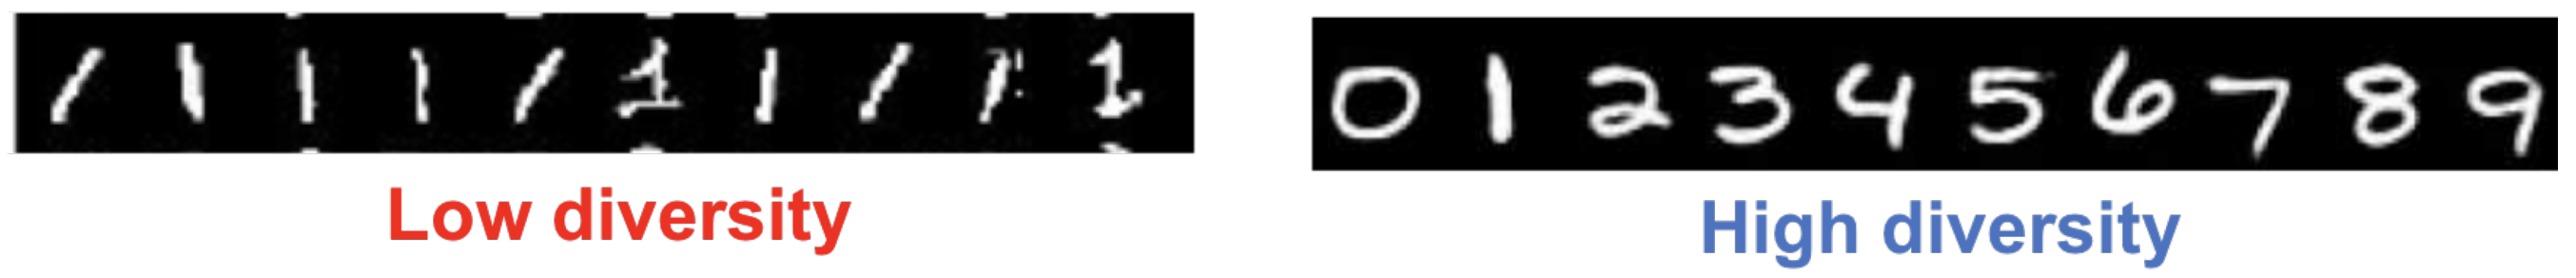
\includegraphics[width=0.9\linewidth]{figs/diversity}
			\end{figure}
		\end{itemize}
	\end{block}
\end{frame}
%=======
\subsection{Frechet Inception Distance (FID)}
%=======
\begin{frame}{Wasserstein Metric}
	\myfootnotewithlink{https://arxiv.org/abs/1706.08500}{Heusel M. et al. GANs Trained by a Two Time-Scale Update Rule Converge to a Local Nash Equilibrium, 2017}
	\vspace{-0.2cm}
	\[
		W_s(\pi \| p) = \inf_{\gamma \in \Gamma(\pi, p)} \left(\bbE_{(\bx_1, \bx_2) \sim \gamma} \| \bx_1 - \bx_2 \|^s\right)^{1/s}
	\]
	\eqpause
	\vspace{-0.3cm}
	\begin{block}{Wasserstein GAN (Optimal Transport)}
		\vspace{-0.5cm}
		{\small
		\[
			W(\pi \| p) = \inf_{\gamma \in \Gamma(\pi, p)} \bbE_{(\bx_1, \bx_2) \sim \gamma} \| \bx_1 - \bx_2 \| =  \inf_{\gamma\in {\Gamma(\pi, p)}} \int { \| \bx_1 - \bx_2 \|} {\gamma (\bx_1, \bx_2)} d \bx_1 d \bx_2
		\]
		}
		\vspace{-0.5cm}
	\end{block}
	\eqpause
	\begin{block}{Theorem}
		If $\pi(\bx) = \cN(\bmu_\pi, \bSigma_\pi)$, $p(\bx) = \cN(\bmu_p, \bSigma_p)$, then
		\vspace{-0.2cm}
		\[
			W_2^2(\pi \| p) = \| \bmu_{\pi} - \bmu_{p}\|^2 + \text{tr} \left[ \bSigma_{\pi} + \bSigma_p - 2 \left(\bSigma_{\pi}^{1/2} \bSigma_p \bSigma_{\pi}^{1/2} \right)^{1/2} \right]
		\]
		\vspace{-0.7cm}
	\end{block}
	\eqpause
	\begin{block}{Frechet Inception Distance}
		\vspace{-0.3cm}
		\[
			\FID (\pd, \pt) =  W_2^2(\pd \| \pt)
		\]
		\vspace{-0.6cm}
	\end{block}
\end{frame}
%=======
\begin{frame}{Frechet Inception Distance (FID)}
	\myfootnotewithlink{https://arxiv.org/abs/2401.09603}{Jayasumana S. et al. Rethinking FID: Towards a Better Evaluation Metric for Image Generation, 2024}
	\vspace{-0.3cm}
	\[
		\FID (\pd, \pt) = \| \bmu_{\text{data}} - \bmu_{\boldsymbol{\theta}}\|^2 + \text{tr} \left[ \bSigma_{\text{data}} + \bSigma_{\boldsymbol{\theta}} - 2 \left(\bSigma_{\text{data}}^{1/2} \bSigma_{\boldsymbol{\theta}} \bSigma_{\text{data}}^{1/2} \right)^{1/2} \right]
	\]
	\vspace{-0.5cm}
	\begin{itemize}
		\item FID is computed in the latent space $\bz$.
		\item We use a pretrained image embedder to get latent representations $\bz = \bff(\bx)$.
		\item $\bmu_{\text{data}}$, $\bSigma_{\text{data}}$ and $\bmu_{\boldsymbol{\theta}}$, $\bSigma_{\boldsymbol{\theta}}$ are statistics of latent representations for samples from $\pd(\bx)$ and $\pt(\bx)$.
	\end{itemize}
	\eqpause
	\begin{block}{$FID(p(\bx), \cN(0, \bI))$}
		\begin{figure}
			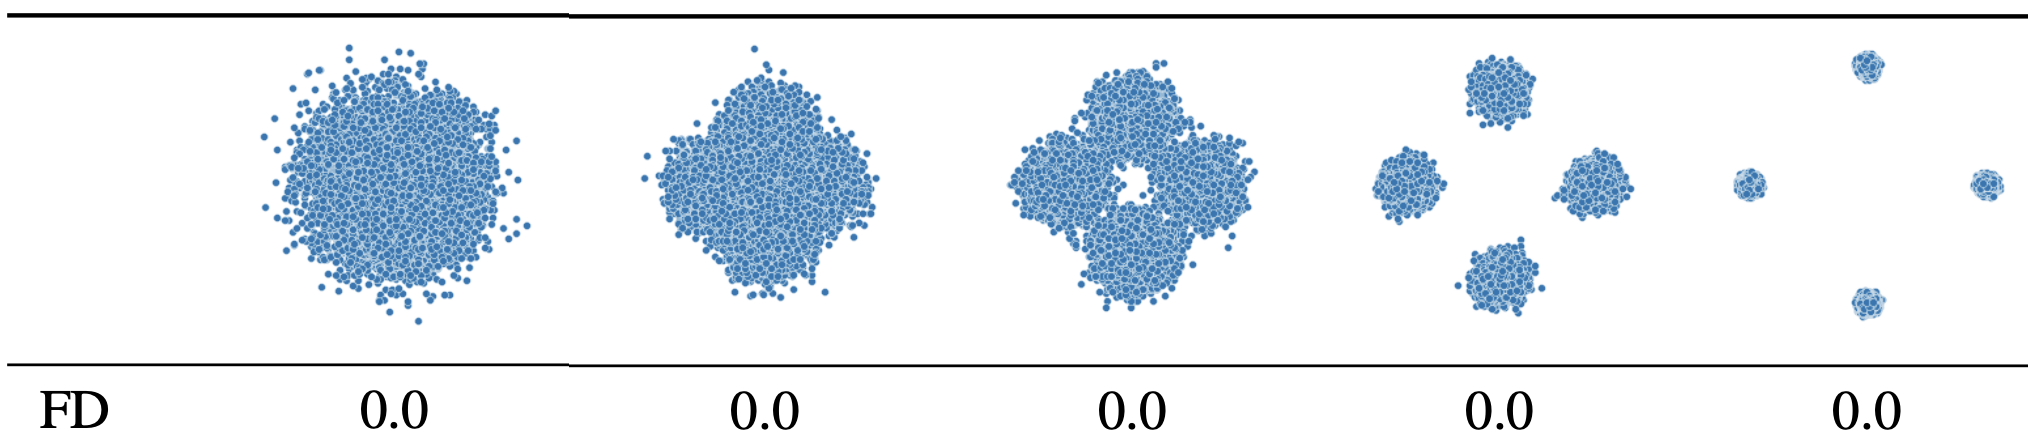
\includegraphics[width=0.95\linewidth]{figs/fid_normal}
		\end{figure}
	\end{block}
\end{frame}
%=======
\begin{frame}{Frechet Inception Distance (FID)}
	\myfootnotewithlink{https://arxiv.org/abs/2401.09603}{Jayasumana S. et al. Rethinking FID: Towards a Better Evaluation Metric for Image Generation, 2024}
	\vspace{-0.4cm}
	\[
		\FID (\pd, \pt) = \| \bmu_{\text{data}} - \bmu_{\boldsymbol{\theta}}\|^2 + \text{tr} \left[ \bSigma_{\text{data}} + \bSigma_{\boldsymbol{\theta}} - 2 \left(\bSigma_{\text{data}}^{1/2} \bSigma_{\boldsymbol{\theta}} \bSigma_{\text{data}}^{1/2} \right)^{1/2} \right]
	\]
	\eqpause
	\vspace{-0.3cm}
	\begin{block}{Drawbacks}
		\begin{itemize}
			\item Depends on the pretrained classification network.
			\item Uses the normality assumption.
			\item May not correlate with human evaluation.
		\end{itemize}
	\end{block}
	\begin{figure}
		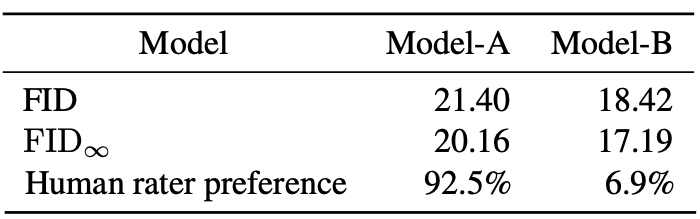
\includegraphics[width=0.7\linewidth]{figs/fid_vs_human_eval}
	\end{figure}
\end{frame}
%=======
\subsection{Precision-Recall}
%=======
\begin{frame}{Precision-Recall}
	\myfootnotewithlink{https://arxiv.org/abs/1904.06991}{Kynkäänniemi T. et al. Improved precision and recall metric for assessing generative models, 2019}
	\vspace{-0.5cm}
	\begin{block}{Desirable Properties for Samples}
		\begin{itemize}
			\item \textbf{Sharpness}: generated samples should possess high visual quality.
			\item \textbf{Diversity}: their variation should match that in the training data.
		\end{itemize}
	\end{block}
	\eqpause
	\vspace{-0.5cm}
	\begin{figure}
		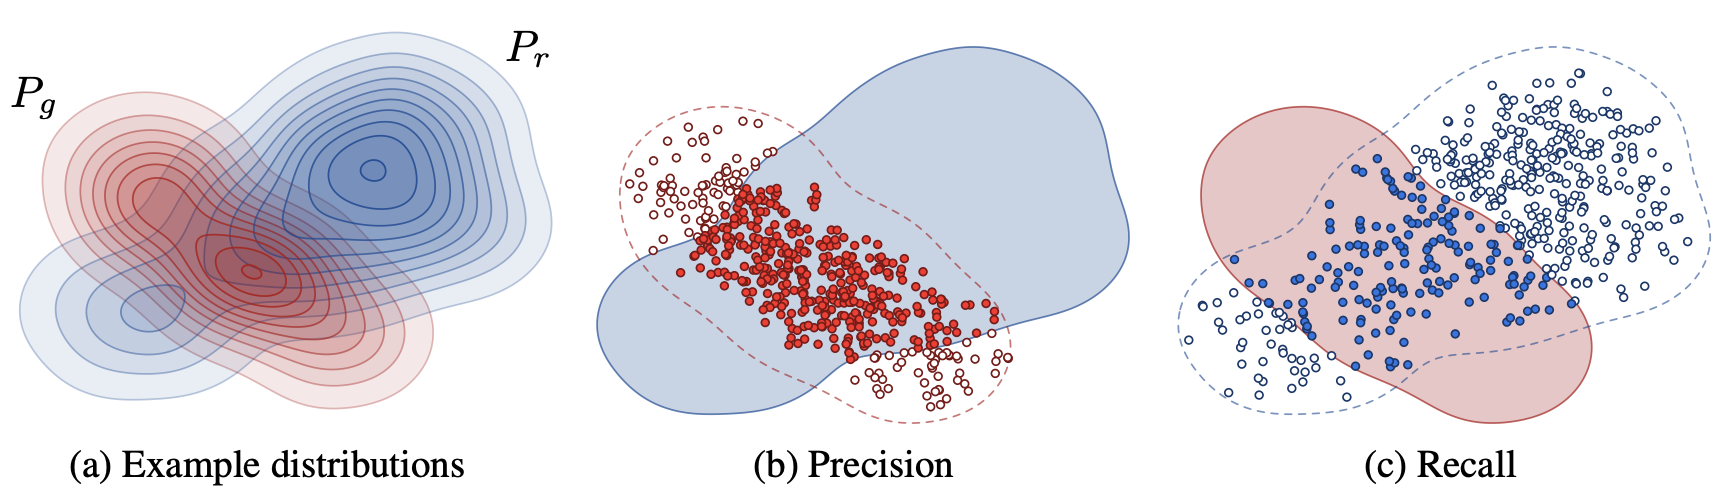
\includegraphics[width=0.9\linewidth]{figs/pr_curve}
	\end{figure}
	\vspace{-0.3cm}
	\begin{itemize}
		\item \textbf{Precision} denotes the fraction of generated images that look realistic.
		\item \textbf{Recall} measures how well the generator covers the training data manifold.
	\end{itemize}
\end{frame}
%=======
\begin{frame}{Precision-Recall}
	\myfootnotewithlink{https://arxiv.org/abs/1904.06991}{Kynkäänniemi T. et al. Improved precision and recall metric for assessing generative models, 2019}
	\vspace{-0.2cm}
	\begin{itemize}
		\item $\cS_{\text{data}} = \{\bx_i\}_{i=1}^{n} \sim \pd(\bx)$ -- real samples;
		\item $\cS_{\btheta} = \{\bx_i\}_{i=1}^{n} \sim \pt(\bx)$ -- generated samples.
	\end{itemize}
	\eqpause
	Define a binary function:
	\vspace{-0.2cm}
	\[
		\bbI(\bx, \cS) =
		\begin{cases}
			1, & \text{if } \exists\ \bx' \in \cS: \| \bx - \bx'\|_2 \leq \| \bx' - \text{NN}_k(\bx', \cS)\|_2; \\
			0, & \text{otherwise.}
		\end{cases}
	\]
	\eqpause
	\vspace{-0.3cm}
	\[
		\text{Pr} (\cS_{\text{data}}, \cS_{\btheta}) = \frac{1}{n} \sum_{\bx \in \cS_{\btheta}} \bbI(\bx, \cS_{\text{data}}); \quad \text{Rec} (\cS_{\text{data}}, \cS_{\btheta}) = \frac{1}{n} \sum_{\bx \in \cS_{\text{data}}} \bbI(\bx, \cS_{\btheta}).
	\]
	\eqpause
	\vspace{-0.6cm}
	\begin{figure}
		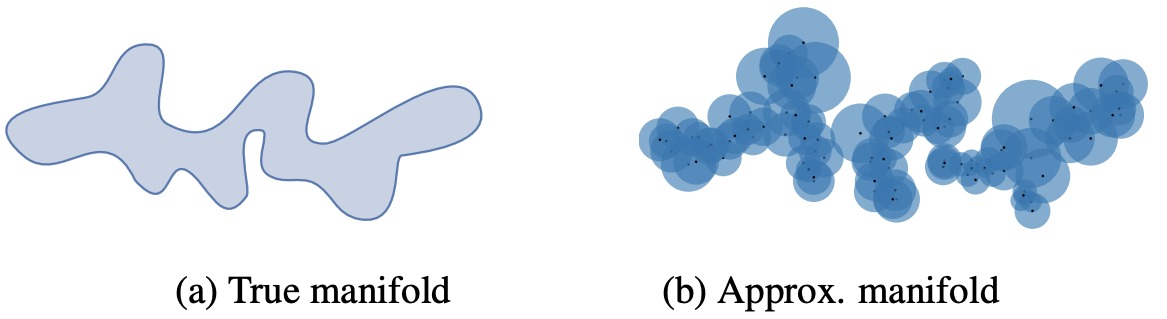
\includegraphics[width=0.75\linewidth]{figs/pr_k_nearest}
	\end{figure}
	\eqpause
	Embed the samples using a pretrained network (as in FID).
\end{frame}
%=======
\begin{frame}{Precision-Recall}
	\myfootnotewithlink{https://arxiv.org/abs/1904.06991}{Kynkäänniemi T. et al. Improved precision and recall metric for assessing generative models, 2019}
	\vspace{-0.3cm}
	\begin{figure}
		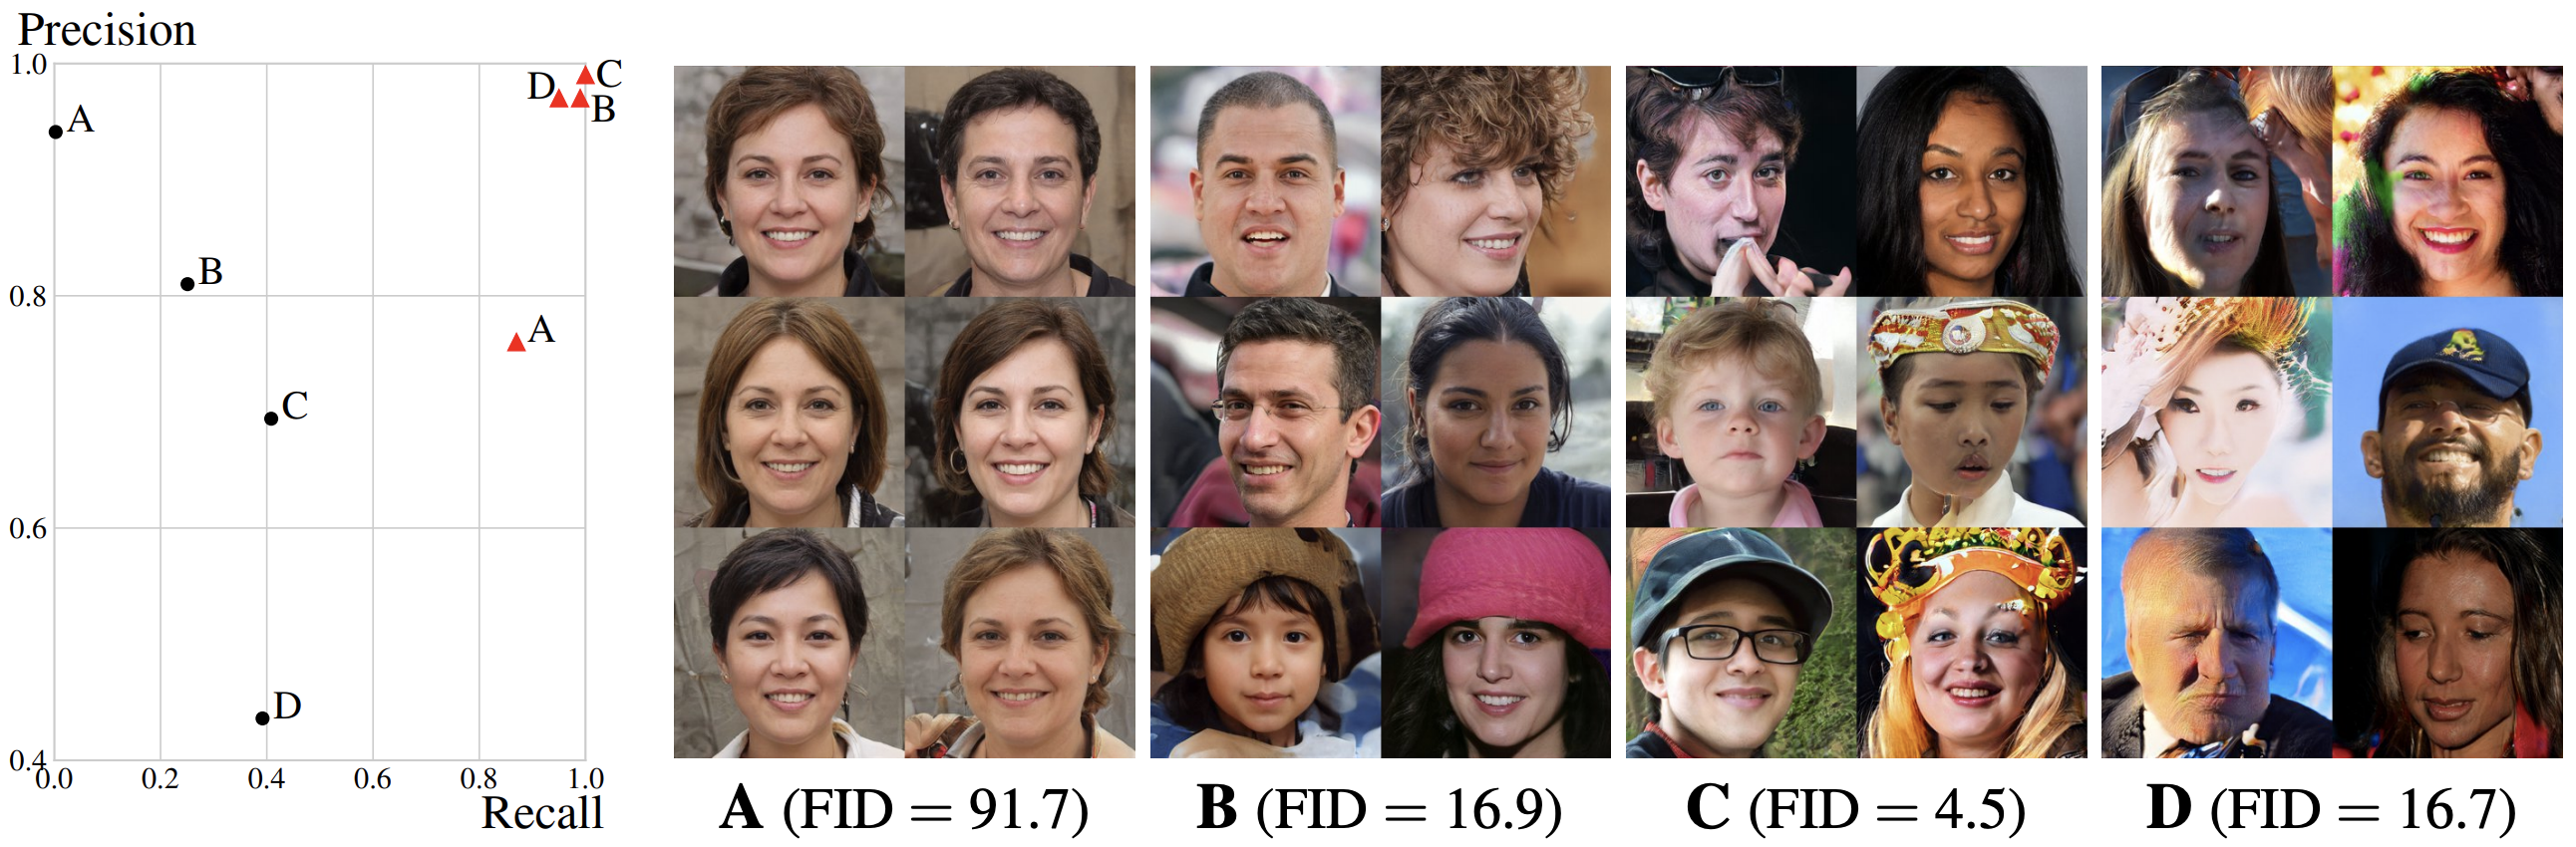
\includegraphics[width=\linewidth]{figs/pr_vs_fid}
	\end{figure}
	\eqpause
	\vspace{-0.3cm}
	\begin{figure}
		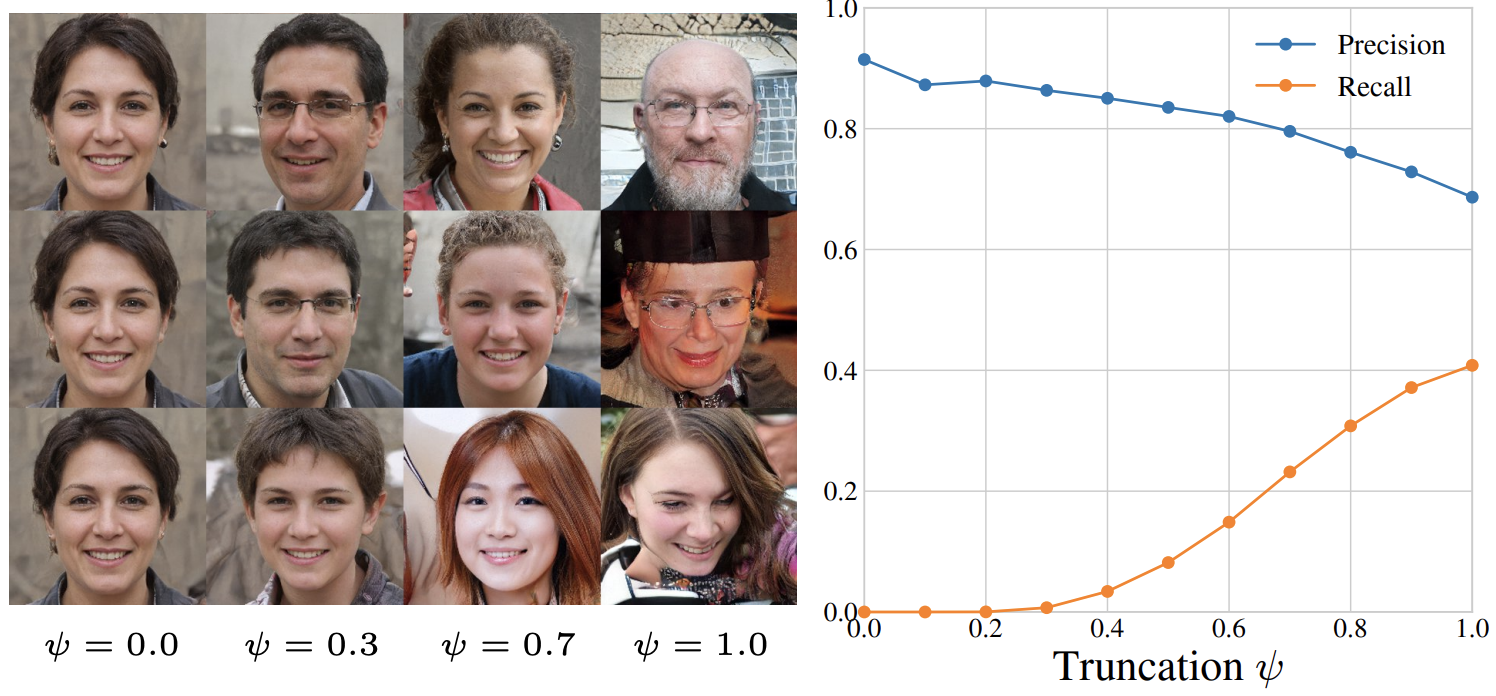
\includegraphics[width=0.75\linewidth]{figs/pr_truncation}
	\end{figure}
\end{frame}
%=======
\subsection{CLIP Score}
%=======
\begin{frame}{CLIP Score}
	\myfootnotewithlink{https://arxiv.org/abs/2103.00020}{Radford A. et al. Learning transferable visual models from natural language supervision, 2021} 
	\vspace{-0.5cm}
	\begin{minipage}{0.5\linewidth}
		\begin{block}{Unconditional Model}
			\begin{figure}
				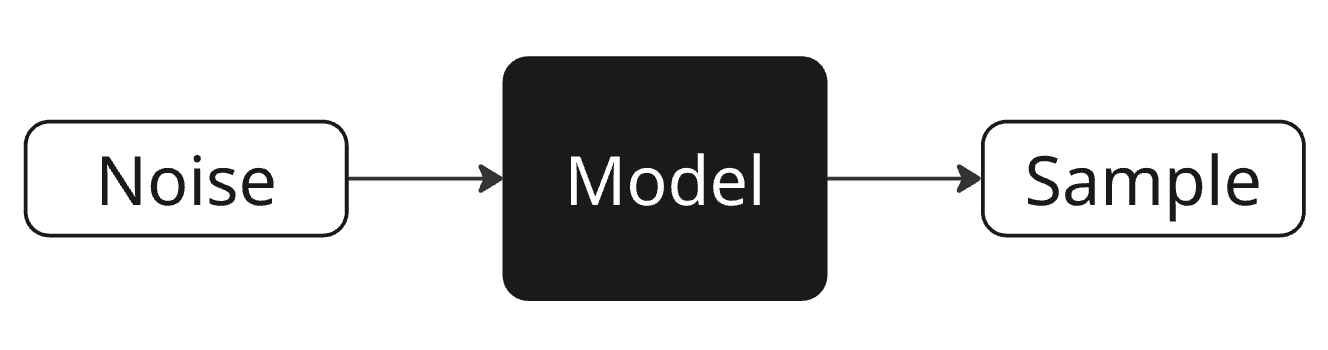
\includegraphics[width=0.95\linewidth]{figs/uncond_model}
			\end{figure}
		\end{block}
		\vspace{0.2cm}
	\end{minipage}%
	\begin{minipage}{0.5\linewidth}
		\begin{block}{Conditional Model}
			\begin{figure}
				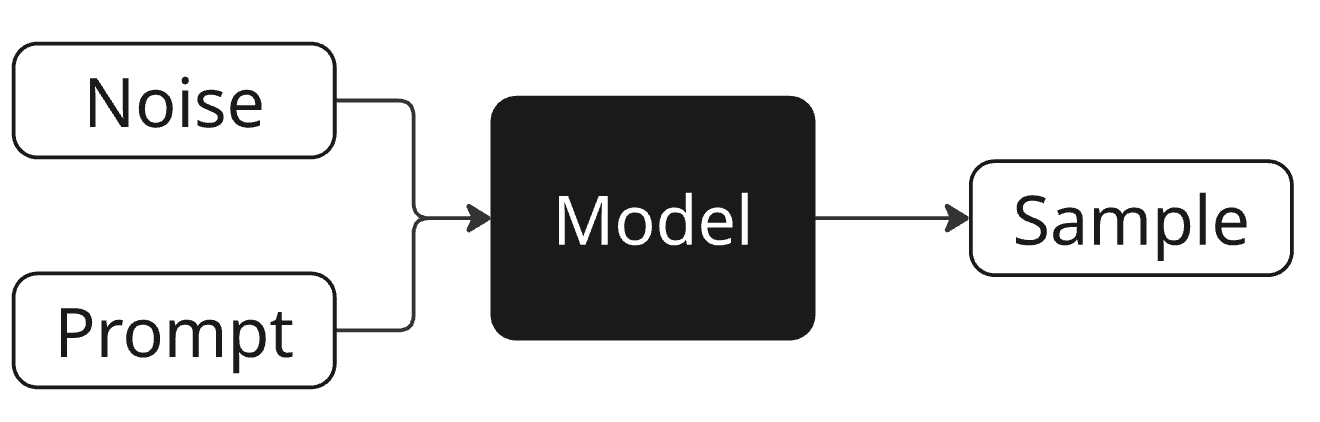
\includegraphics[width=0.95\linewidth]{figs/cond_model}
			\end{figure}
		\end{block}
	\end{minipage}

	\eqpause
	We need a way to measure not only the quality of the generated image, but also how well it's aligned with the prompt.
	\eqpause
	\begin{figure}
		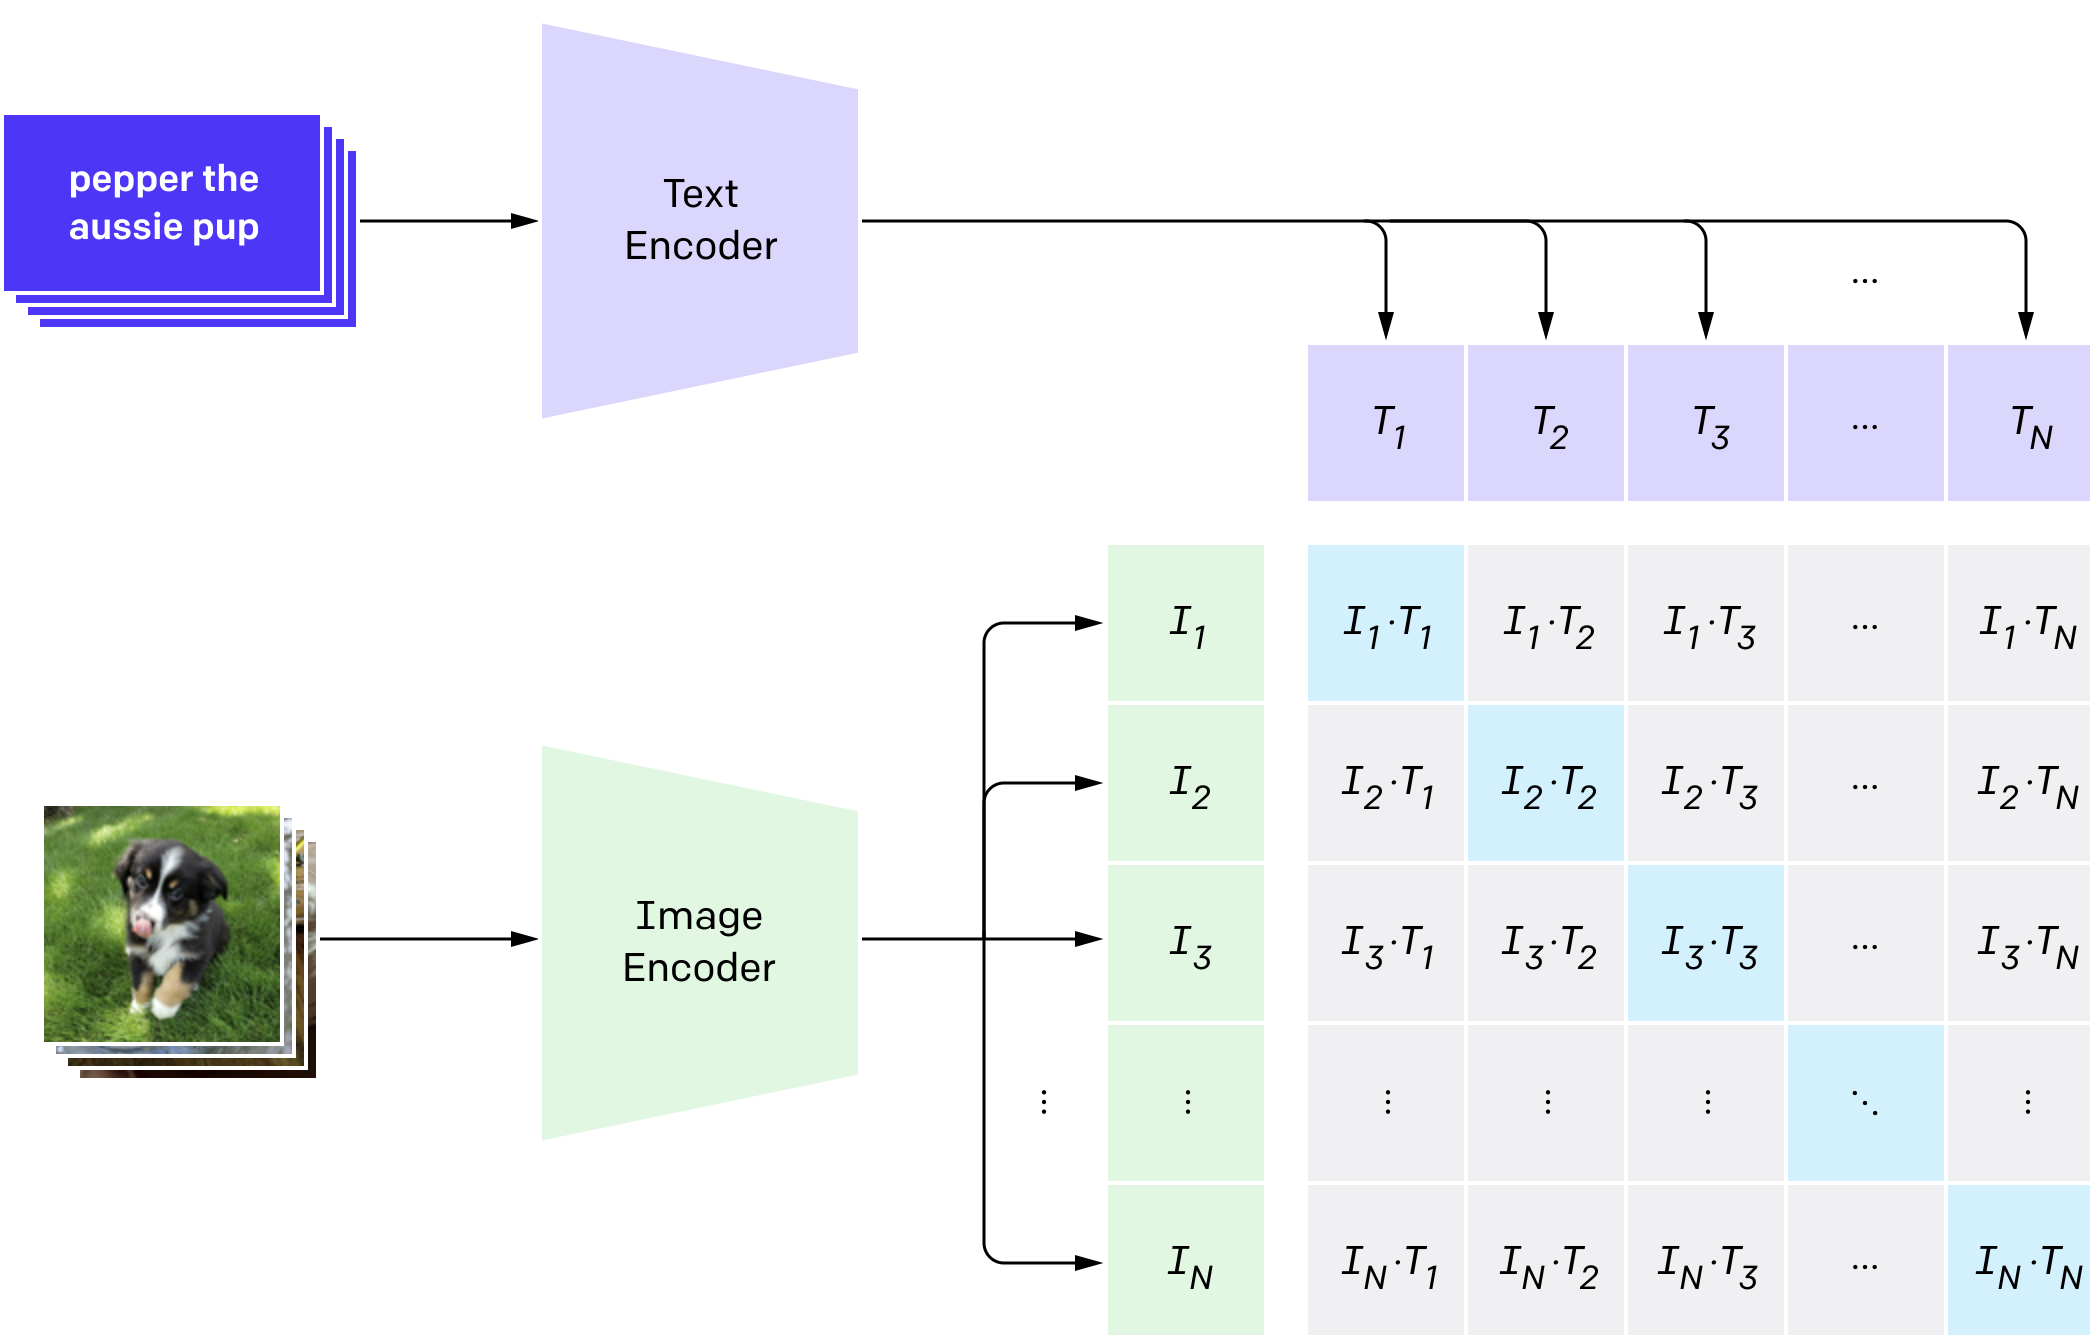
\includegraphics[width=0.6\linewidth]{figs/clip}
	\end{figure}
\end{frame}
%=======
\subsection{Human Evaluation}
%=======
\begin{frame}{Human Evaluation}
	\myfootnotewithlink{https://ya.ru/ai/art}{YandexART 2.5, 2025} 
	\begin{itemize}
		\item No automated metric is perfect.
		\item The best way to evaluate generative models is by human assessment.
		\item It's important to assess various properties.
	\end{itemize}
	\eqpause
	\begin{figure}
		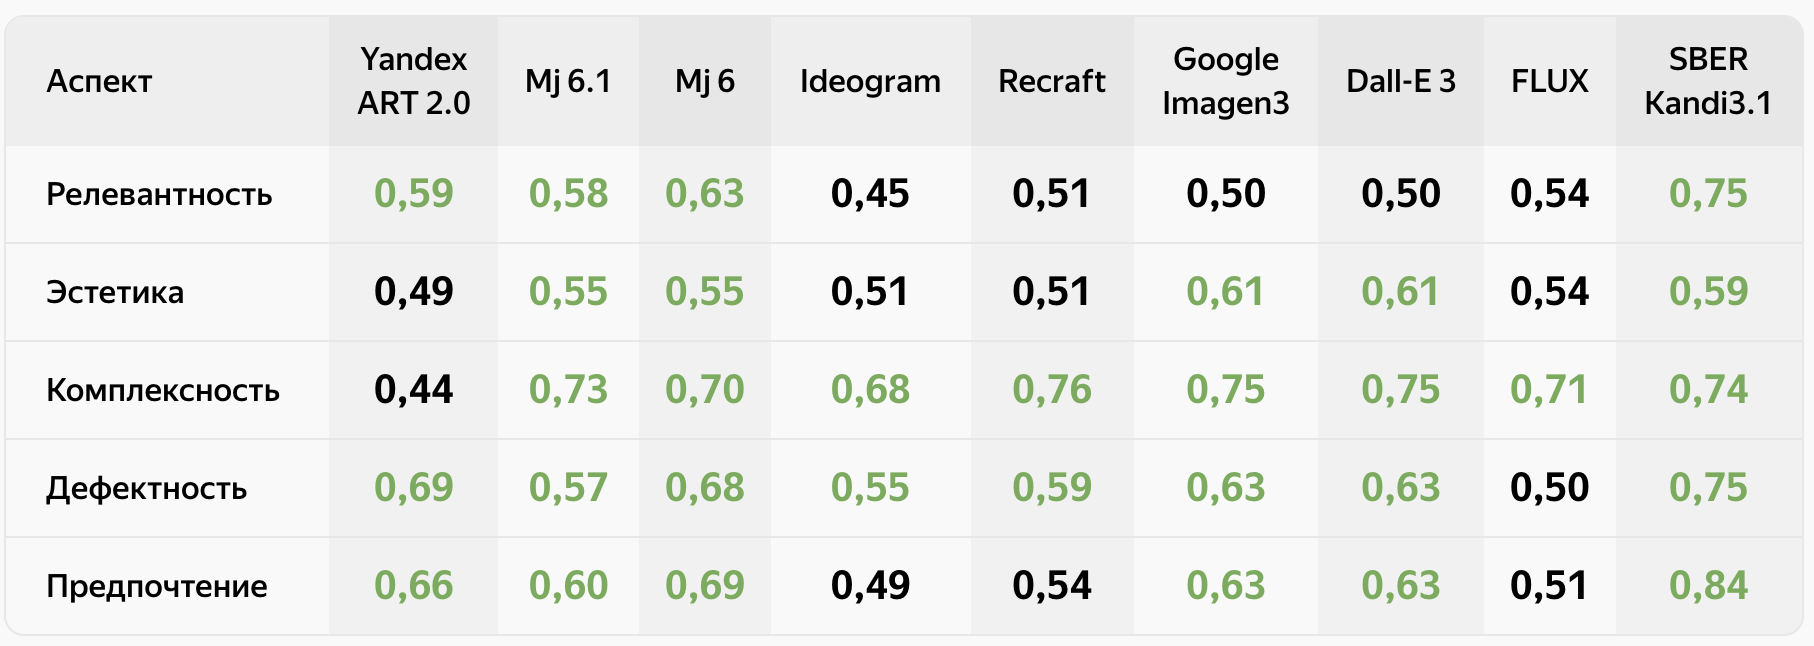
\includegraphics[width=1.0\linewidth]{figs/yaart_2.5}
	\end{figure}
\end{frame}
%=======
\section{Langevin Dynamics}
%=======
\begin{frame}{Energy-Based Models}
	\begin{block}{Unnormalized Density}
		\vspace{-0.2cm}
		\[
			\pt(\bx) = \frac{\hat{p}_{\btheta}(\bx)}{Z_{\btheta}}, \quad \text{where } Z_{\btheta} = \int \hat{p}_{\btheta}(\bx) d \bx
		\]
		\vspace{-0.3cm}
		\begin{itemize}
			\item $\hat{p}_{\btheta}(\bx)$ can be any non-negative function. \\
			\item If we reparameterize as $\hat{p}_{\btheta}(\bx) = \exp(-f_{\btheta}(\bx))$, we eliminate the non-negativity constraint.
		\end{itemize}
	\end{block}
	\eqpause
	\vspace{-0.3cm}
	\begin{block}{Unnormalized Density}
		The gradient of the normalized log-density equals that of the unnormalized log-density:
		\[
			\nabla_{\bx} \log \pt(\bx) = \nabla_{\bx} \log \hat{p}_{\btheta}(\bx) - \nabla_{\bx} \log Z_{\btheta} = \nabla_{\bx} \log \hat{p}_{\btheta}(\bx)
		\]
	\end{block}
	\eqpause
	\vspace{-0.3cm}
	\begin{itemize}
		\item Suppose we already have this density (normalized or not) $\pt(\bx)$.
		\item How can we sample from the model?
	\end{itemize}
\end{frame}
%=======
\begin{frame}{Langevin Dynamics}
	\myfootnotewithlink{https://arxiv.org/abs/1704.04752}{Dalalyan A. Further and stronger analogy between sampling and optimization: Langevin Monte Carlo and gradient descent, 2017.}
	\begin{block}{Theorem}
		Consider energy-based model $p(\bx) = \frac{\hat{p}(\bx)}{Z}$, $\hat{p}(\bx) = \exp(-f(\bx))$, with continuously differentiable $f(\bx): \bbR^m \rightarrow \bbR$ that satisfies
		\begin{itemize}
			\item $L$-smoothness: $\| \nabla f(\bx) - \nabla f(\by)\| \leq L \|\bx - \by \|$;
			\item Strong convexity: $(\nabla f(\bx) - \nabla f(\by))^T(\bx - \by) \geq m \| \bx - \by \|^2 $ for some $m > 0$.
		\end{itemize}
		Consider a Markov chain $\bx_{l + 1} = \bx_l + \frac{\eta}{2} \cdot \nabla_{\bx_l} \log \hat{p}(\bx_l) + \sqrt{\eta} \cdot \bepsilon_l$, where $\bepsilon_l \sim \cN(0, \bI)$.
		Then, for any $\eta < \frac{2}{L}$
		\begin{itemize}
			\item The Markov chain has a unique stationary distribution $\pi_\eta$.
			\item $W_2(\pi_\eta, p) \le C \eta$, and as $\eta \to 0$ we have $\pi_\eta \xrightarrow{d} p$.
		\end{itemize}
	\end{block}
\end{frame}
%=======
\begin{frame}{Langevin Dynamics}
	\myfootnotewithlink{https://yang-song.github.io/blog/2021/score/}{Song Y. Generative Modeling by Estimating Gradients of the Data Distribution, blog post, 2021}
	\vspace{-0.4cm}
	\begin{block}{Theorem (Informal)}
		Let $\bx_0$ be a random vector. Under mild regularity conditions, samples from the following dynamics will eventually follow $\pt(\bx)$ (for sufficiently small $\eta$ and large $l$):
		\vspace{-0.3cm}
		\[
			\bx_{l + 1} = \bx_l + \frac{\eta}{2} \cdot \nabla_{\bx_l} \log \pt(\bx_l) + \sqrt{\eta} \cdot \bepsilon_l, \quad \bepsilon_l \sim \cN(0, \bI).
		\]
		\vspace{-0.5cm}
	\end{block}
	\eqpause
	\begin{minipage}{0.55\linewidth}
		\begin{itemize}
			\item What if $\bepsilon_l = \boldsymbol{0}$?
			\item The density $\pt(\bx)$ is the \textbf{stationary} distribution of the Markov chain.
			\item The gradient is taken with respect to $\bx$, not $\btheta$.
			\item $\nabla_{\bx} \log \pt(\bx)$ defines a vector field.
		\end{itemize}
	\end{minipage}%
	\begin{minipage}{0.45\linewidth}
		\begin{figure}
			\centering
			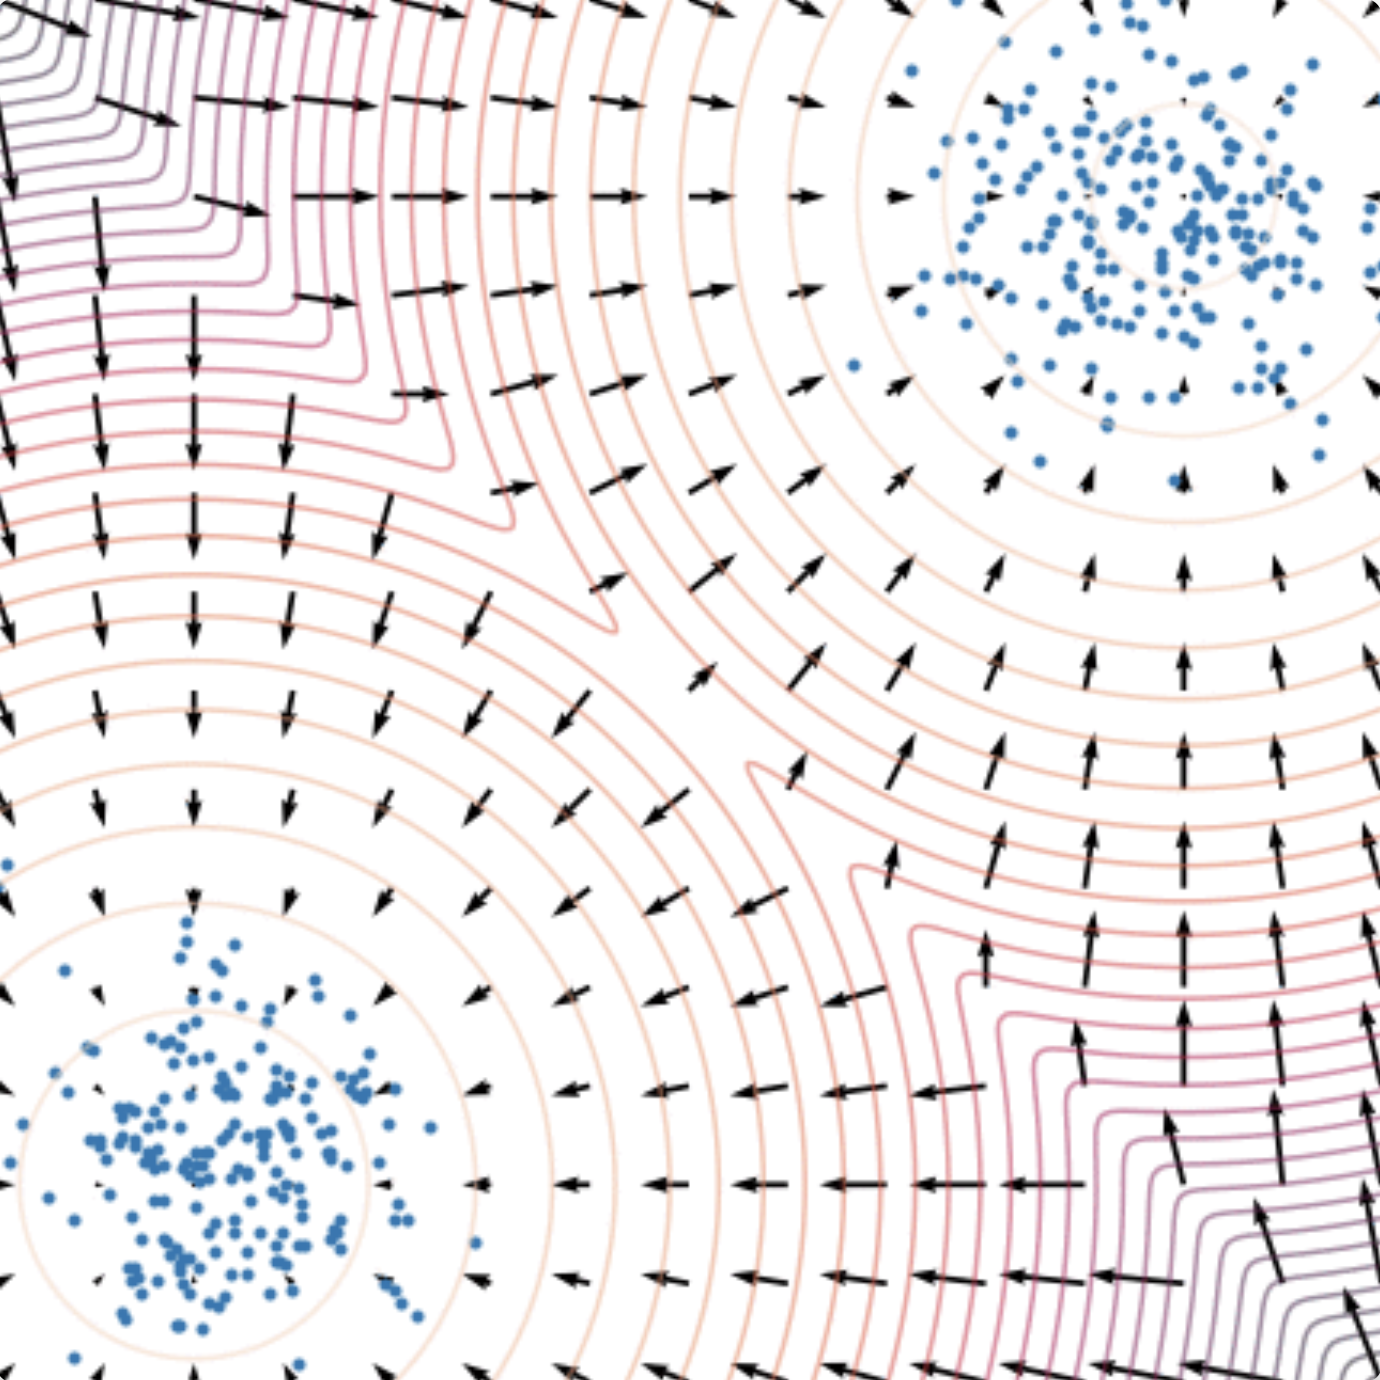
\includegraphics[width=0.9\linewidth]{figs/langevin_dynamic}
		\end{figure}
	\end{minipage}
\end{frame}
%=======
\section{Score Matching}
%=======
\begin{frame}{Score Matching}
	\myfootnotewithlink{https://yang-song.github.io/blog/2021/score/}{Song Y. Generative Modeling by Estimating Gradients of the Data Distribution, blog post, 2021}
	\begin{block}{Score Function}
		\vspace{-0.3cm}
		 \[
			 \bs_{\btheta}(\bx) = \nabla_{\bx}\log \pt(\bx)
		 \]
		\vspace{-0.5cm}
	\end{block}
	\eqpause
	\begin{block}{Langevin Dynamics}
		If we know the score function $\bs_{\btheta}(\bx) = \nabla_{\bx}\log \pt(\bx)$, we can generate samples from the model using Langevin dynamics:
		\[
			\bx_{l + 1} = \bx_l + \frac{\eta}{2} \cdot {\color{violet}\nabla_{\bx_l} \log \pt(\bx_l)} + \sqrt{\eta} \cdot \bepsilon_l = \bx_l + \frac{\eta}{2} \cdot {\color{violet}\bs_{\btheta}(\bx_l)} + \sqrt{\eta} \cdot \bepsilon_l.
		\]
		\vspace{-0.5cm}
	\end{block}
	\eqpause
	\begin{block}{Fisher Divergence}
		\vspace{-0.7cm}
		\begin{multline*}
			D_F(\pd, \pt) = \frac{1}{2}\bbE_{\pi}\big\| \nabla_{\bx}\log \pt(\bx) - \nabla_\bx \log \pd(\bx) \big\|^2_2 =\\
			= \frac{1}{2}\bbE_{\pi}\big\| \bs_{\btheta}(\bx) - \nabla_\bx \log \pd(\bx) \big\|^2_2 \rightarrow \min_{\btheta}
		\end{multline*}
		\vspace{-0.3cm}
	\end{block}
\end{frame}
%=======
\begin{frame}{Score Matching}
	\myfootnotewithlink{https://yang-song.github.io/blog/2021/score/}{Song Y. Generative Modeling by Estimating Gradients of the Data Distribution, blog post, 2021}
	\begin{block}{Fisher Divergence}
		\vspace{-0.3cm}
		\[
			D_F(\pd, \pt) = \frac{1}{2}\bbE_{\pi}\big\| \bs_{\btheta}(\bx) - \nabla_\bx \log \pd(\bx) \big\|^2_2 \rightarrow \min_{\btheta}
		\]
		\vspace{-0.5cm}
	\end{block}
	\begin{figure}
		\centering
		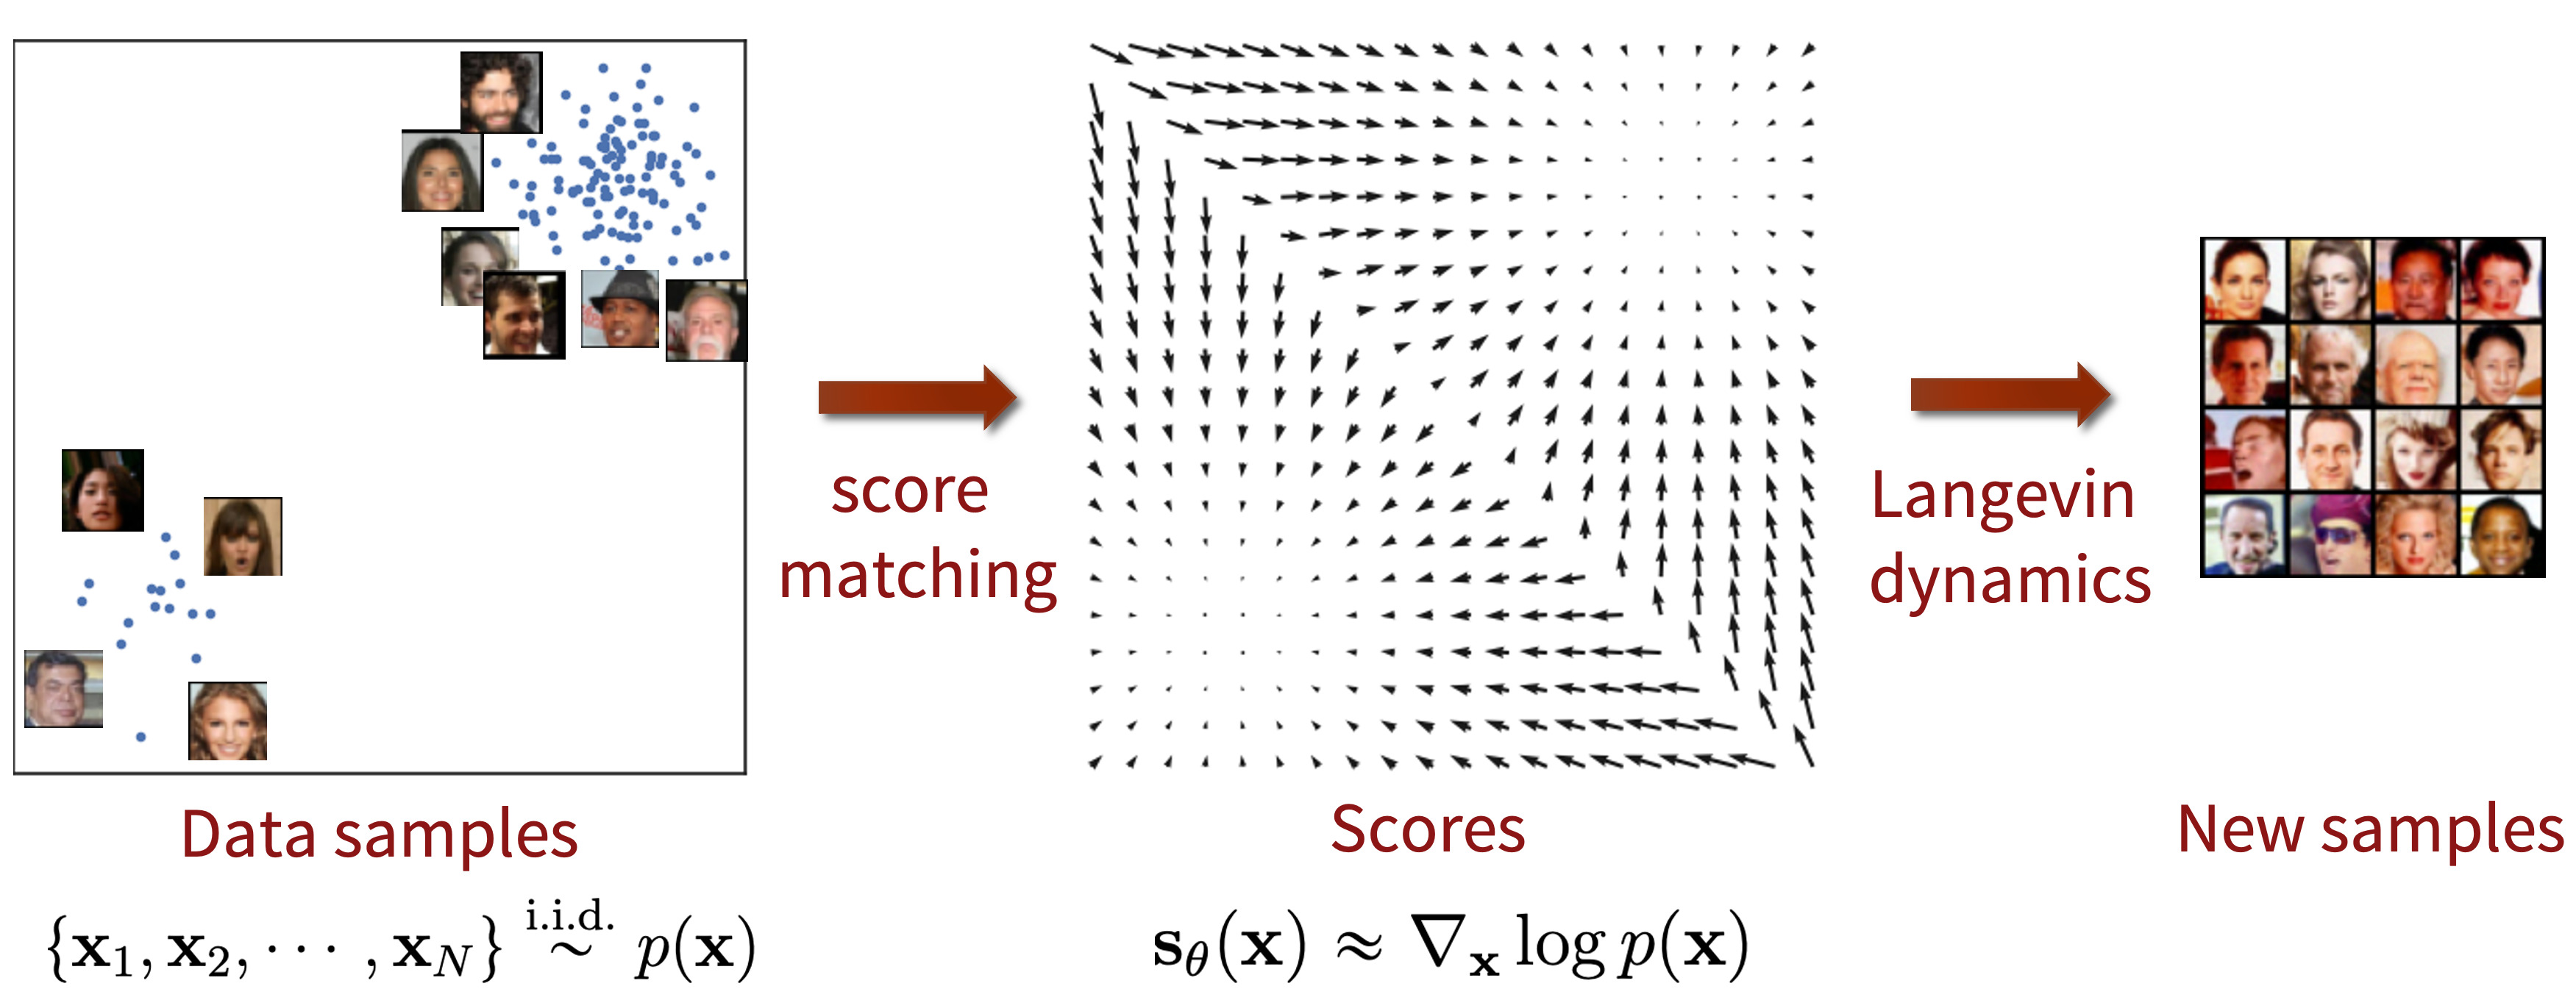
\includegraphics[width=\linewidth]{figs/smld}
	\end{figure}
	\eqpause
	\textbf{Problem:} We don't know $\nabla_\bx \log \pd(\bx)$.
\end{frame}
%=======
\section{Denoising Score Matching}
%=======
\begin{frame}{Denoising Score Matching}
	\myfootnotewithlink{http://www.iro.umontreal.ca/~vincentp/Publications/smdae_techreport.pdf}{Vincent P. A Connection Between Score Matching and Denoising Autoencoders, 2010}

	Let us perturb the original data $\bx \sim \pd(\bx)$ with Gaussian noise:
	\vspace{-0.3cm}
	\[
		\bx_{\sigma} = \bx + \sigma \cdot \bepsilon, \quad \bepsilon \sim \cN(0, \bI), \quad q(\bx_{\sigma} | \bx) = \cN(\bx, \sigma^2 \cdot \bI)
	\]
	\eqpause
	\vspace{-0.4cm}
	\[
		q(\bx_{\sigma}) = \int q(\bx_{\sigma} | \bx) \pd(\bx) d\bx.
	\]
	\eqpause
	\vspace{-0.5cm}
	\begin{block}{Assumption}
		The solution to
		\[
			\frac{1}{2} \bbE_{q(\bx_{\sigma})}\big\| \bs_{\btheta, \sigma}(\bx_{\sigma}) - \nabla_{\bx_{\sigma}} \log q(\bx_{\sigma}) \big\|^2_2 \rightarrow \min_{\btheta}
		\]
		\vspace{-0.3cm} \\
		satisfies $\bs_{\btheta, \sigma}(\bx_{\sigma}) \approx \bs_{\btheta, 0}(\bx_0) = \bs_{\btheta}(\bx)$ if $\sigma$ is sufficiently small.
	\end{block}
	\eqpause
	\begin{itemize}
		\item The score function of the noised data nearly matches the score function of the original data.
		\item The score function $\bs_{\btheta, \sigma}(\bx_{\sigma})$ is parameterized by $\sigma$.
		\item \textbf{Note:} We don't know $q(\bx_{\sigma})$, just as we don't know $\pd(\bx)$.
	\end{itemize}
\end{frame}
%=======
\begin{frame}{Denoising Score Matching}
	\myfootnotewithlink{http://www.iro.umontreal.ca/~vincentp/Publications/smdae_techreport.pdf}{Vincent P. A Connection Between Score Matching and Denoising Autoencoders, 2010}
	\begin{block}{Theorem}
		Under mild regularity conditions, the following holds:
		\vspace{-0.3cm}
		\begin{multline*}
			\bbE_{q(\bx_{\sigma})}\big\| \bs_{\btheta, \sigma}(\bx_{\sigma}) - \nabla_{\bx_{\sigma}} \log q(\bx_{\sigma}) \big\|^2_2 = \\
		= \bbE_{\pd(\bx)} \bbE_{q(\bx_{\sigma} | \bx)}\big\| \bs_{\btheta, \sigma}(\bx_{\sigma}) - \nabla_{\bx_{\sigma}} \log q(\bx_{\sigma} | \bx) \big\|^2_2 + \text{const}(\btheta)
		\end{multline*}
		\vspace{-0.5cm}
	\end{block}
	\eqpause
	\begin{block}{Gradient of the Noise Kernel}
		\vspace{-0.3cm}
		\[
			\bx_{\sigma} = \bx + \sigma \cdot \bepsilon, \quad q(\bx_{\sigma} | \bx) = \cN(\bx, \sigma^2 \cdot \bI)
		\]
		\eqpause
		\vspace{-0.3cm}
		\[
			\nabla_{\bx_{\sigma}} \log q(\bx_{\sigma} | \bx) = - \frac{\bx_{\sigma} - \bx}{\sigma^2}  = - \frac{\bepsilon}{\sigma}
		\]
		\eqpause
		\vspace{-0.5cm}
	\end{block}
	\begin{itemize}
		\item The right-hand side doesn't require computing $\nabla_{\bx_{\sigma}} \log q(\bx_{\sigma})$ or even $\nabla_{\bx_{\sigma}} \log \pd(\bx_{\sigma})$.
		\item $\bs_{\btheta, \sigma}(\bx_{\sigma})$ is trained to \textbf{denoise} the noised samples $\bx_{\sigma}$.
	\end{itemize}
\end{frame}
%=======
\begin{frame}{Denoising Score Matching}
	\myfootnotewithlink{https://yang-song.github.io/blog/2021/score/}{Song Y. Generative Modeling by Estimating Gradients of the Data Distribution, blog post, 2021}
	Initial objective:
	\vspace{-0.2cm}
	\[
		\bbE_{\pd(\bx)}\big\| \bs_{\btheta}(\bx) - \nabla_\bx \log \pd(\bx) \big\|^2_2 \rightarrow \min_{\btheta}
	\]
	\eqpause
	\vspace{-0.5cm} \\
	Noised objective:
	\vspace{-0.2cm}
	\[
		\bbE_{q(\bx_{\sigma})}\big\| \bs_{\btheta, \sigma}(\bx_\sigma) - \nabla_\bx \log q(\bx_{\sigma}) \big\|^2_2 \rightarrow \min_{\btheta}
	\]
	\eqpause
	\vspace{-0.5cm} \\
	This is equivalent to a denoising task:
	\vspace{-0.2cm}
	\[
		\bbE_{\pd(\bx)} \bbE_{q(\bx_{\sigma} | \bx)}\big\| \bs_{\btheta, \sigma}(\bx_{\sigma}) - \nabla_{\bx_{\sigma}} \log q(\bx_{\sigma} | \bx) \big\|^2_2 \rightarrow \min_{\btheta}
	\]
	\eqpause
	\vspace{-0.3cm}
	\[
		\bbE_{\pd(\bx)} \bbE_{\cN(0, \bI)}\left\| \bs_{\btheta, \sigma}(\bx + \sigma \cdot \bepsilon) + \frac{\bepsilon}{\sigma} \right\|^2_2 \rightarrow \min_{\btheta}
	\]
	\vspace{-0.5cm}
	\begin{block}{Langevin Dynamics}
		\vspace{-0.3cm}
		\[
			\bx_{l + 1} = \bx_l + \frac{\eta}{2} \cdot \bs_{\btheta, \sigma}(\bx_l) + \sqrt{\eta} \cdot \bepsilon_l, \quad \bepsilon_l \sim \cN(0, \bI).
		\]
		\vspace{-0.7cm}
	\end{block}
\end{frame}
%=======
\begin{frame}{Summary}
	\begin{itemize}
		\item Frechet Inception Distance is the most popular metric for evaluating implicit generative models.
		\vfill
		\item Precision-recall allows for choosing a model that balances sample quality and diversity.
		\vfill
		\item The CLIP score is widely used to measure text-to-image alignment.
		\vfill
		\item The gold standard for evaluating generated image quality is human assessment.
		\vfill
		\item Langevin dynamics enable sampling from generative models using gradients of the log-likelihood.
		\vfill
		\item Score matching proposes minimizing Fisher divergence to estimate the score function.
		\vfill
		\item Denoising score matching optimizes Fisher divergence on noisy data, making it estimable with samples.
	\end{itemize}
\end{frame}
\end{document}